\vspace{0.8cm}

\section{Resultados}
\subsection{Plotter}

\subsection{Seleccionador de colores}

\subsection{Piano}
El sistema desarrollado logró cumplir satisfactoriamente los objetivos propuestos. Se implementó un piano electrónico basado en el microcontrolador ATmega328P, capaz de reproducir las 12 notas de la escala cromática mediante pulsadores individuales. Cada tecla activa la generación de una frecuencia específica a través del buzzer pasivo, logrando un sonido claro y fácilmente distinguible entre notas.

La comunicación UART fue implementada correctamente, permitiendo el control remoto del sistema desde una interfaz serial. Se configuraron tres comandos principales: \texttt{C1} y \texttt{C2}, utilizados para la reproducción de dos canciones predefinidas almacenadas en memoria, y el comando \texttt{PIANO}, que devuelve al modo manual de ejecución por teclas. El comando \texttt{STOP} no fue implementado debido a limitaciones de tiempo, aunque el sistema mantiene estabilidad y correcta respuesta durante la ejecución de las melodías.

\begin{figure}[H]
    \centering
    \includegraphics[width=0.7\columnwidth]{Anexos/Piano_UART.png}
    \caption{Interacción del piano electrónico mediante comunicación UART, mostrando la recepción de comandos desde el terminal serial. Fuente: elaboración propia.}
    \label{fig:piano_uart}
\end{figure}

\begin{figure}[H]
    \centering
    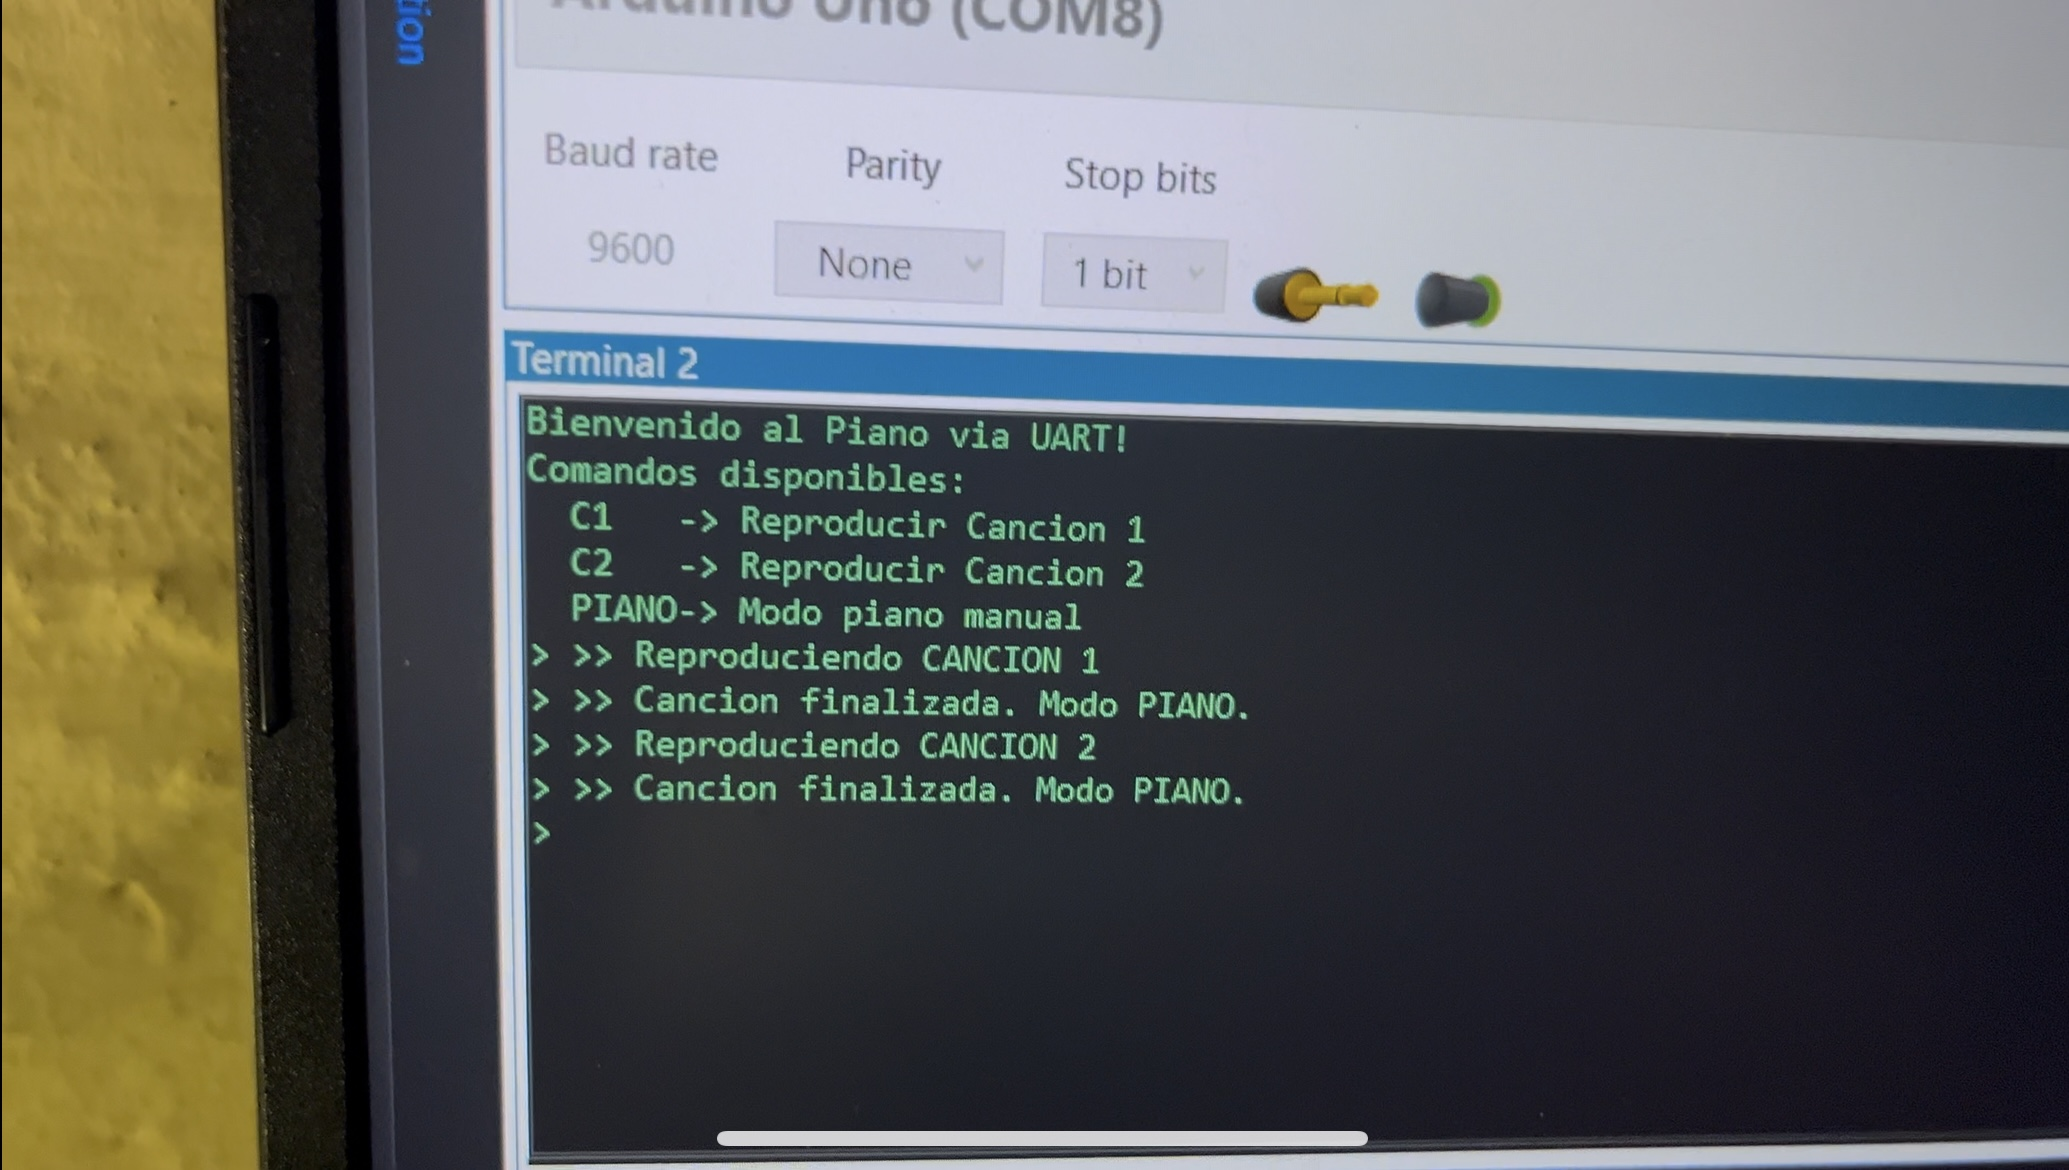
\includegraphics[width=0.7\columnwidth]{Anexos/Piano_Cancion.png}
    \caption{Ejecución automática de una melodía predefinida en el piano electrónico. Fuente: elaboración propia.}
    \label{fig:piano_cancion}
\end{figure}


Durante las pruebas se observó un comportamiento estable en la reproducción de las notas y una respuesta inmediata ante la pulsación de teclas. El buzzer pasivo entregó una calidad sonora adecuada, permitiendo distinguir correctamente las canciones y las frecuencias individuales. No se presentaron problemas de latencia ni de resonancia indebida, confirmando la correcta configuración del temporizador para la generación de las señales PWM.

De forma general, el desempeño del sistema fue considerado satisfactorio, tanto en el modo de ejecución manual como en el automático. Las canciones predefinidas se reprodujeron de forma fluida y reconocible, evidenciando un correcto manejo de tiempos y frecuencias en la modulación del sonido.


\subsection{Cerradura electrónica}

El sistema de cerradura digital presentó un funcionamiento estable y predecible bajo todas las condiciones de prueba. 
Las pruebas experimentales se realizaron en el hardware real, observando tanto la respuesta visual (pantalla LCD y LEDs) 
como la acústica (buzzer), y verificando la coherencia con la lógica definida en el código fuente.

\subsubsection{Validación del PIN}

Durante la fase de ingreso de contraseña, se comprobó que el sistema no permite la validación de PINs con menos de cuatro dígitos, 
mostrando en el LCD el mensaje \texttt{Min 4 digitos} y emitiendo un pitido breve acompañado del encendido del LED rojo.  

\begin{figure}[H]
    \centering
    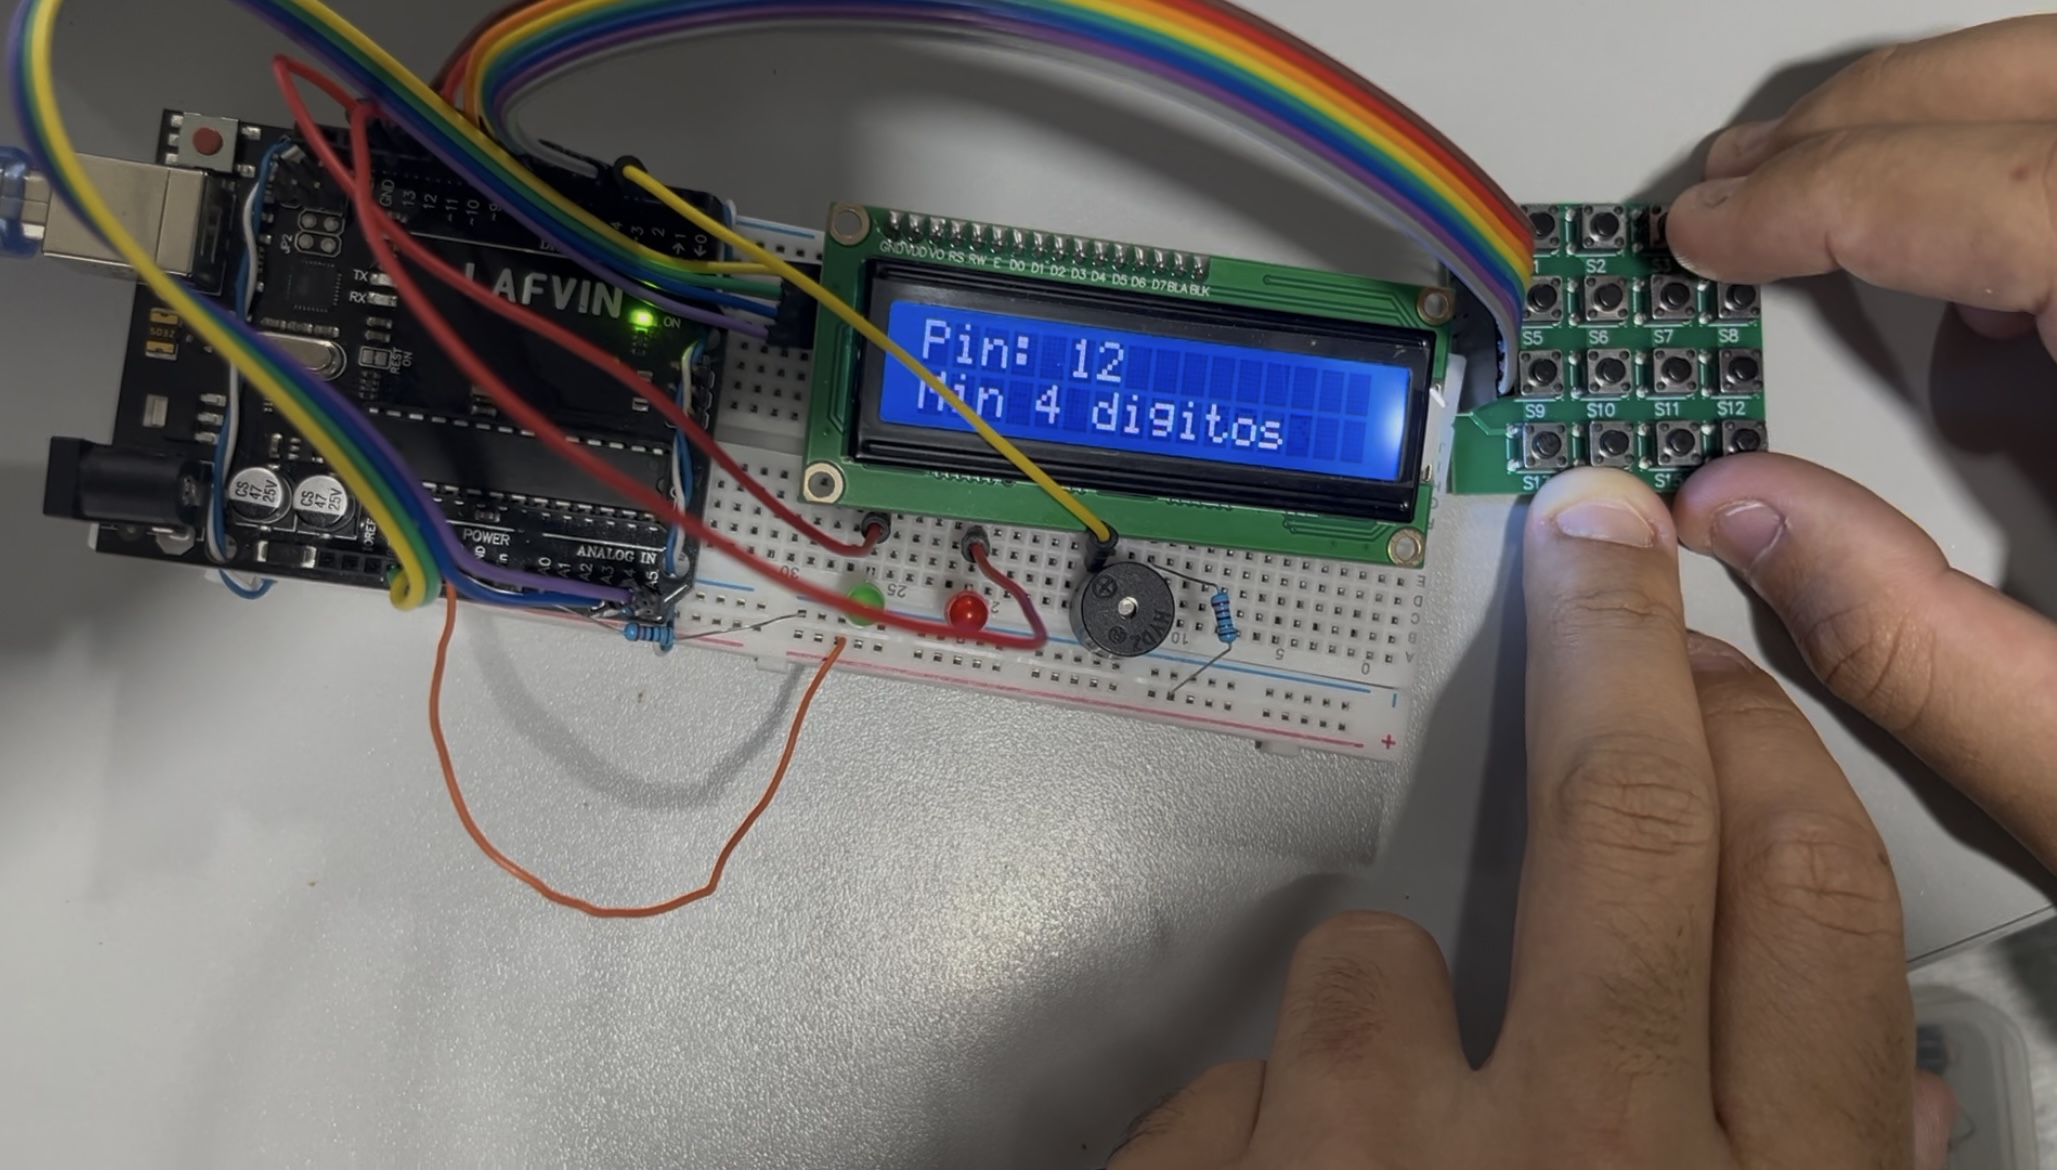
\includegraphics[width=0.7\columnwidth]{Anexos/Cerradura_Min4.png}
    \caption{Mensaje \texttt{Min 4 digitos} mostrado en el LCD y activación del LED rojo al ingresar una contraseña demasiado corta. Fuente: elaboración propia.}
    \label{fig:cerradura_min4}
\end{figure}

Al ingresar un PIN correcto, el sistema reinicia el contador de intentos y activa la señal de confirmación: 
el LED verde se enciende y el buzzer emite tres pulsos cortos, mientras que en la pantalla se muestra el mensaje \texttt{OK}.  

\begin{figure}[H]
    \centering
    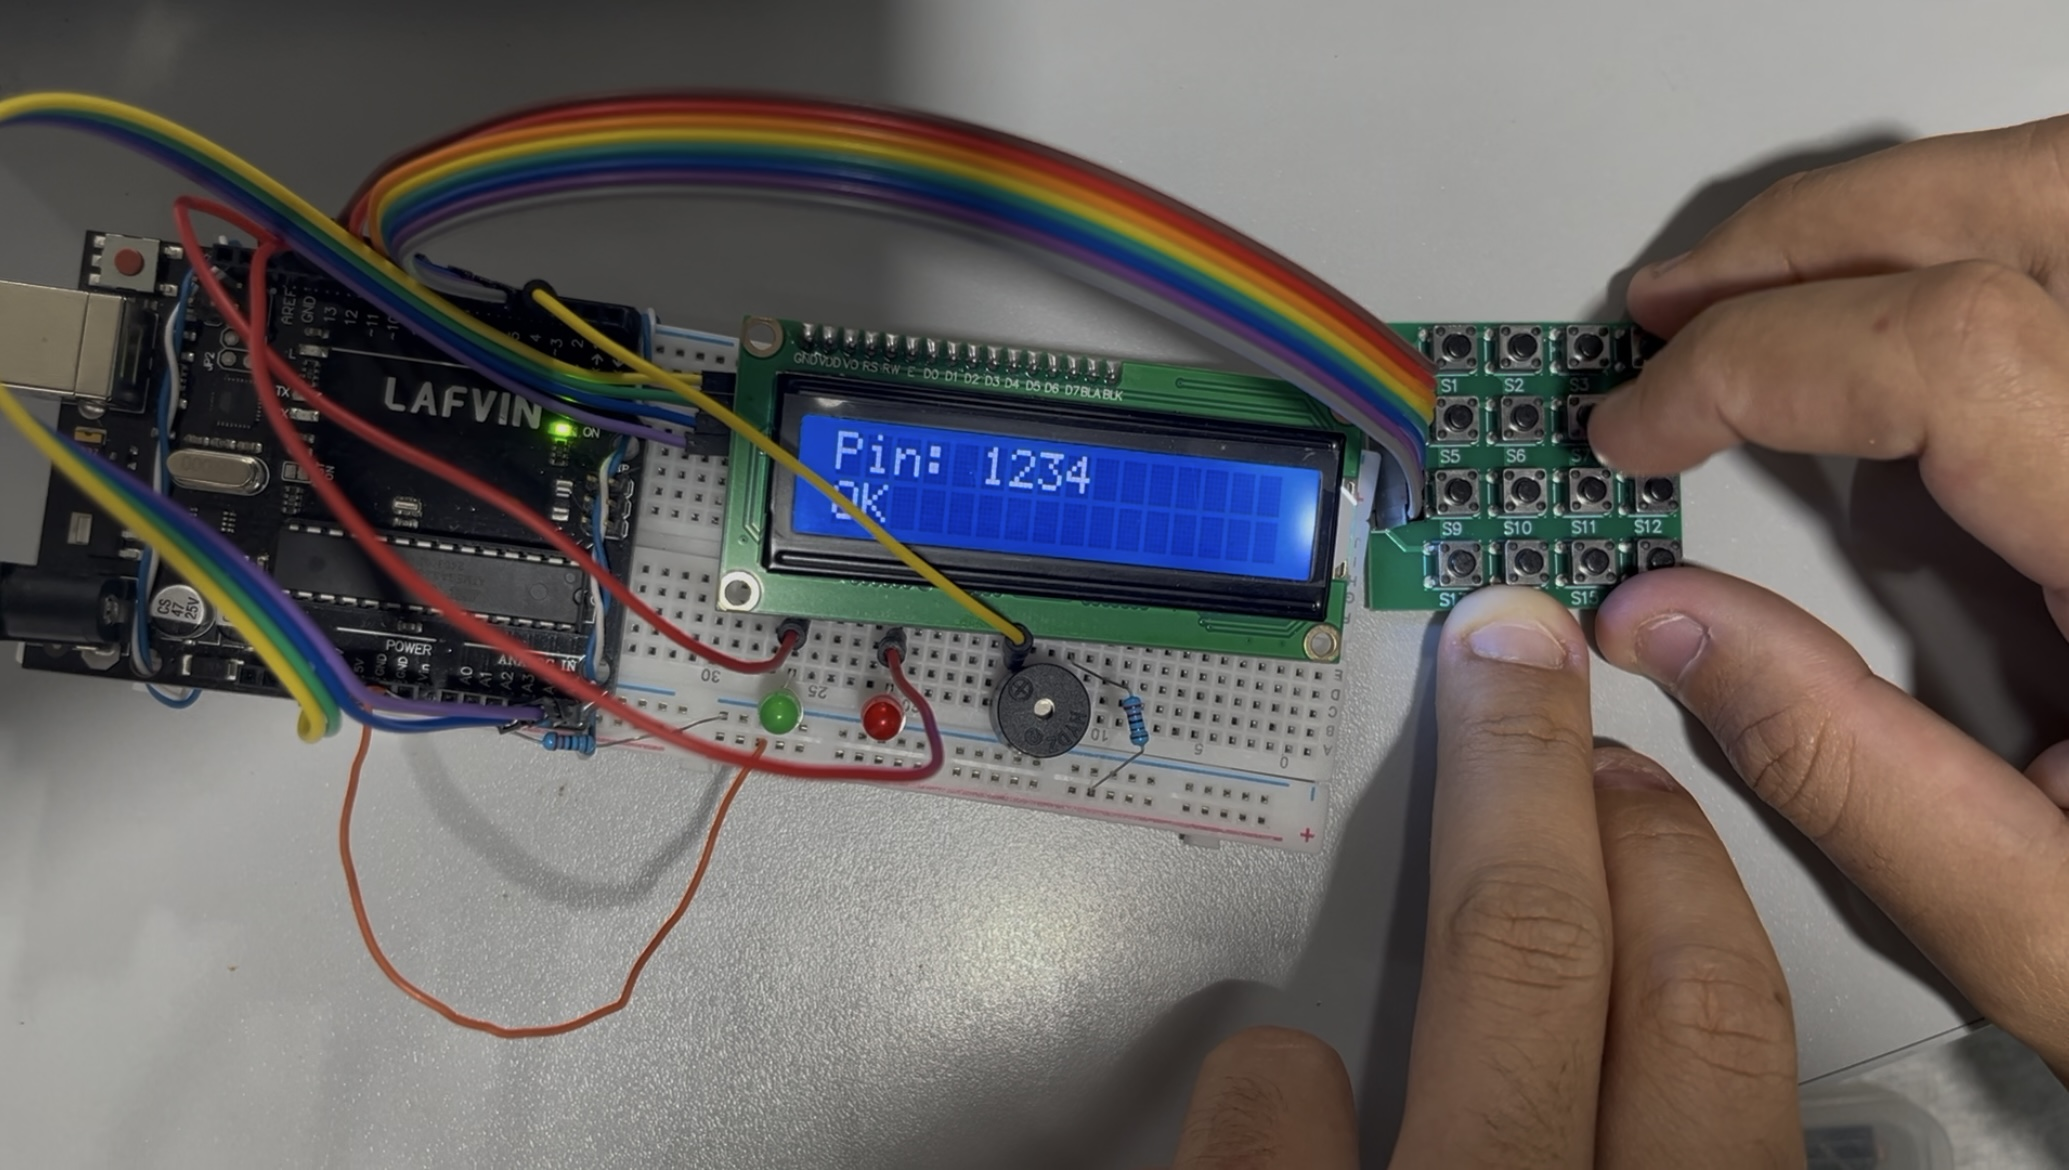
\includegraphics[width=0.7\columnwidth]{Anexos/Cerradura_OK.png}
    \caption{Validación correcta del PIN: mensaje \texttt{OK} en el LCD, LED verde encendido y triple confirmación sonora. Fuente: elaboración propia.}
    \label{fig:cerradura_ok}
\end{figure}

Cuando el PIN es incorrecto, se incrementa el contador de intentos fallidos, 
se activa el LED rojo durante aproximadamente 500~ms junto con un tono continuo en el buzzer, 
y se muestra en el LCD el texto \texttt{Error}.  

\begin{figure}[H]
    \centering
    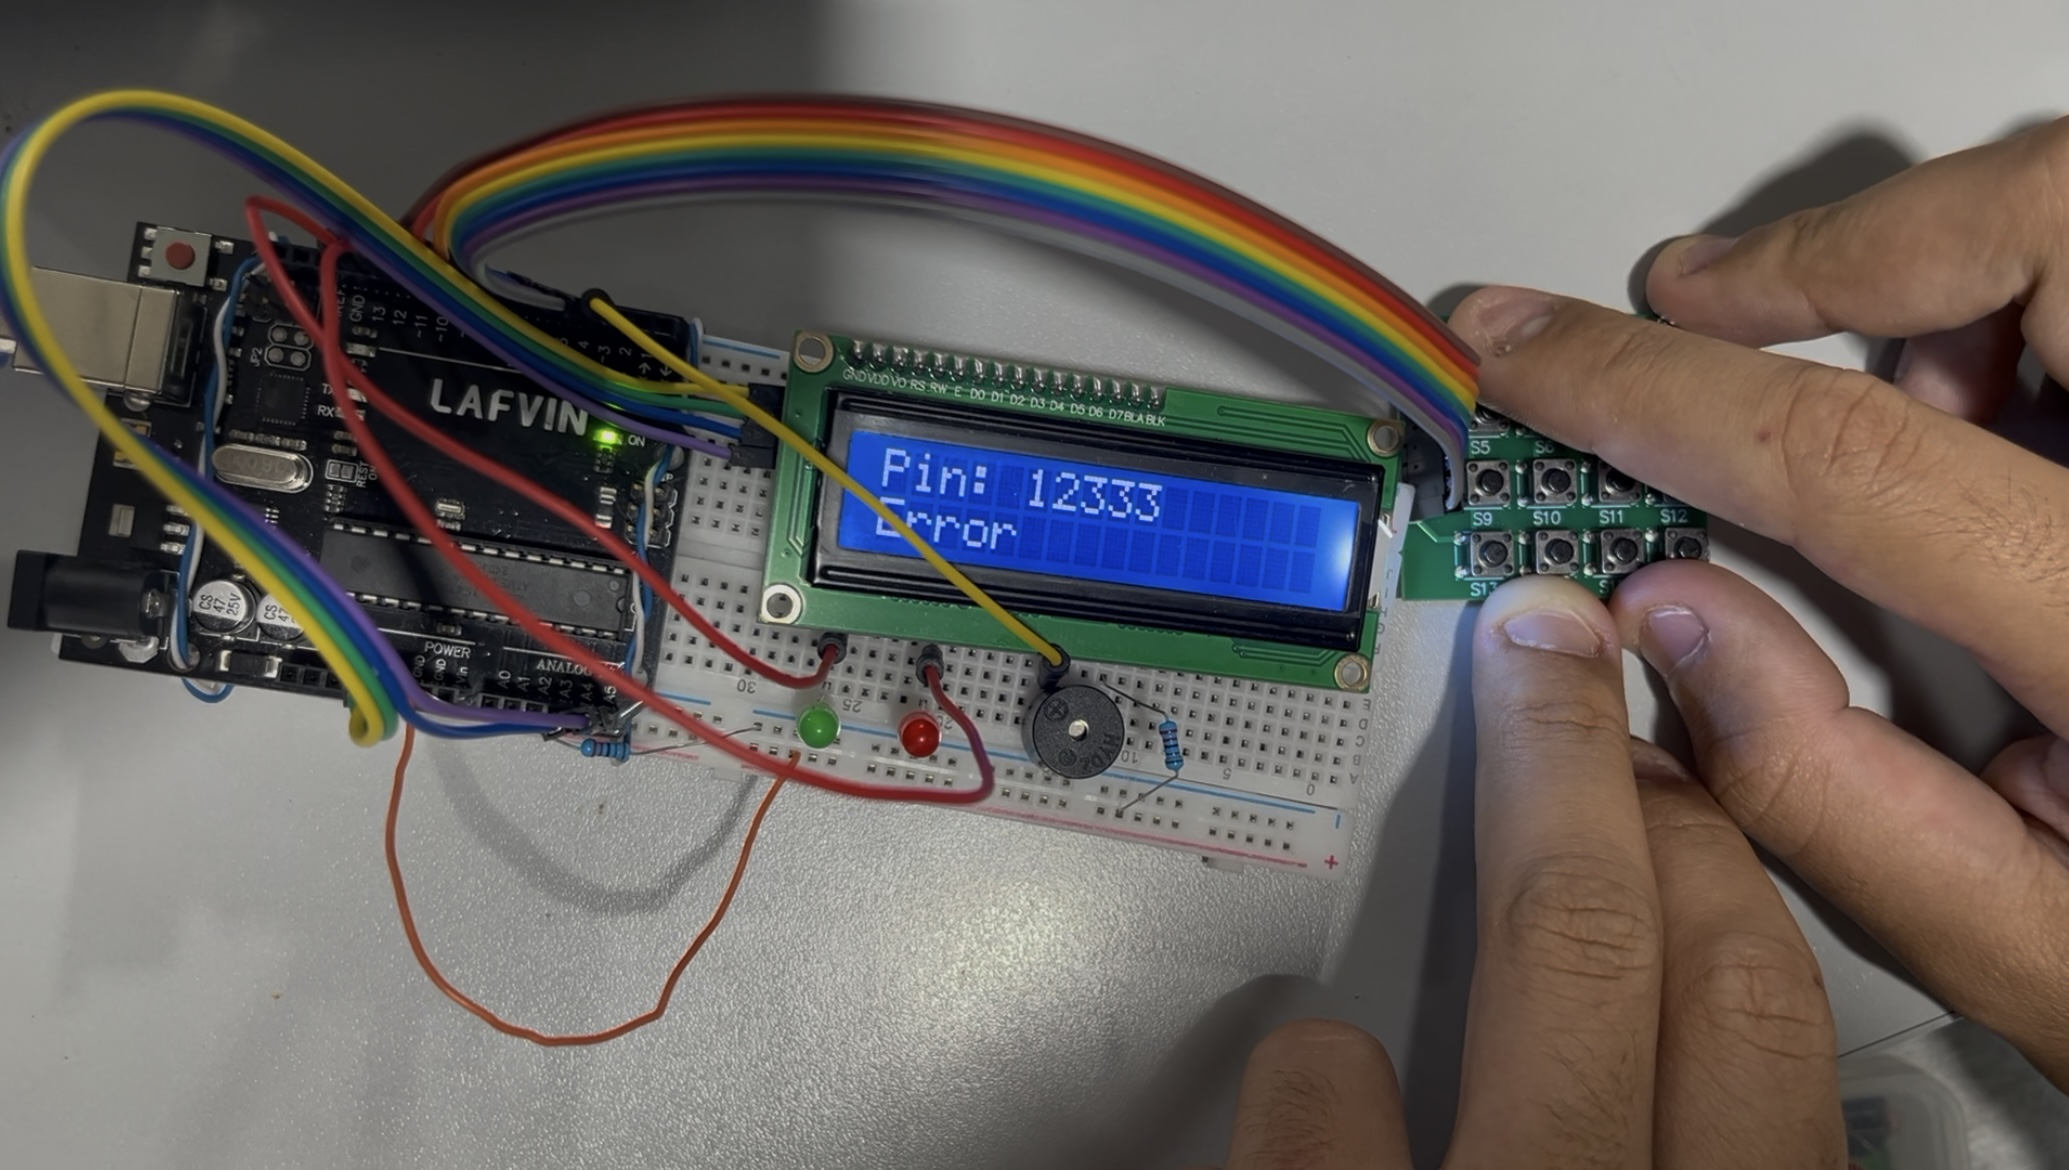
\includegraphics[width=0.7\columnwidth]{Anexos/Cerradura_Error.png}
    \caption{Mensaje \texttt{Error} en el LCD y LED rojo encendido tras ingreso de PIN incorrecto. Fuente: elaboración propia.}
    \label{fig:cerradura_error}
\end{figure}

\subsubsection{Gestión de intentos y bloqueo}

Tras tres intentos consecutivos incorrectos, el sistema ingresa automáticamente en modo de \textbf{bloqueo}.  
En esta condición, el LED rojo y el buzzer alternan su activación de forma intermitente, 
acompañados del mensaje \texttt{Bloqueado} en el LCD.  

\begin{figure}[H]
    \centering
    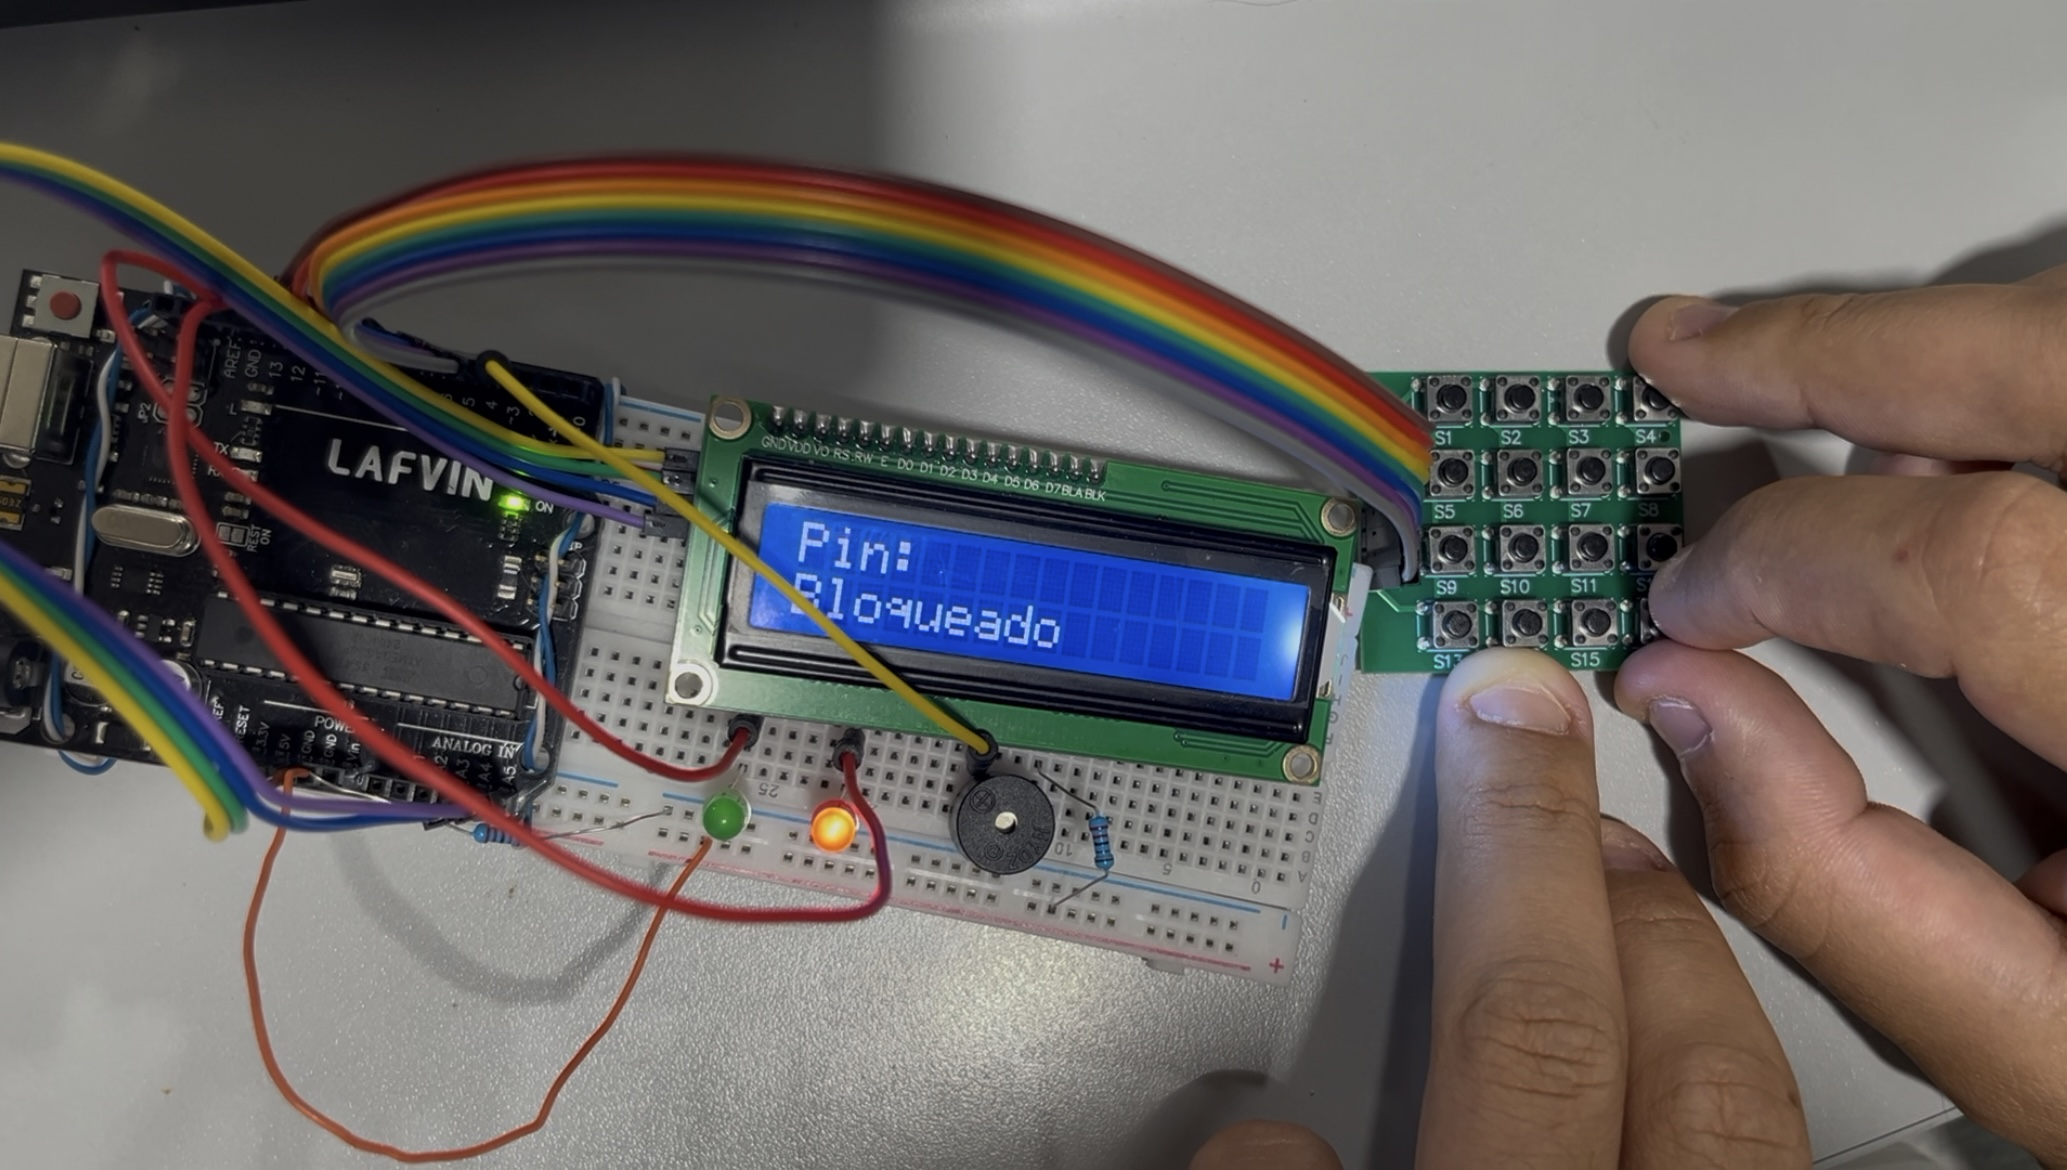
\includegraphics[width=0.7\columnwidth]{Anexos/Cerradura_Bloqueado.png}
    \caption{Estado de bloqueo: mensaje \texttt{Bloqueado} en LCD, LED rojo y buzzer activos. Fuente: elaboración propia.}
    \label{fig:cerradura_bloqueado}
\end{figure}

El bloqueo permanece activo indefinidamente hasta que se presiona la tecla maestra \texttt{D}, 
que actúa como una llave de desbloqueo simbólica.  
Una vez presionada, el sistema apaga las señales de alarma, 
restablece el contador de intentos y retorna al modo normal de operación, mostrando el mensaje \texttt{Listo}.

\subsubsection{Cambio de PIN}

Se verificó correctamente el proceso de modificación de la contraseña utilizando la tecla \texttt{C} para iniciar la secuencia.  
El sistema solicita primero el PIN actual y valida su coincidencia con el valor almacenado en la EEPROM.  
Si es correcto, solicita el nuevo PIN (entre 4 y 6 dígitos) y luego una segunda confirmación.  

\begin{figure}[H]
    \centering
    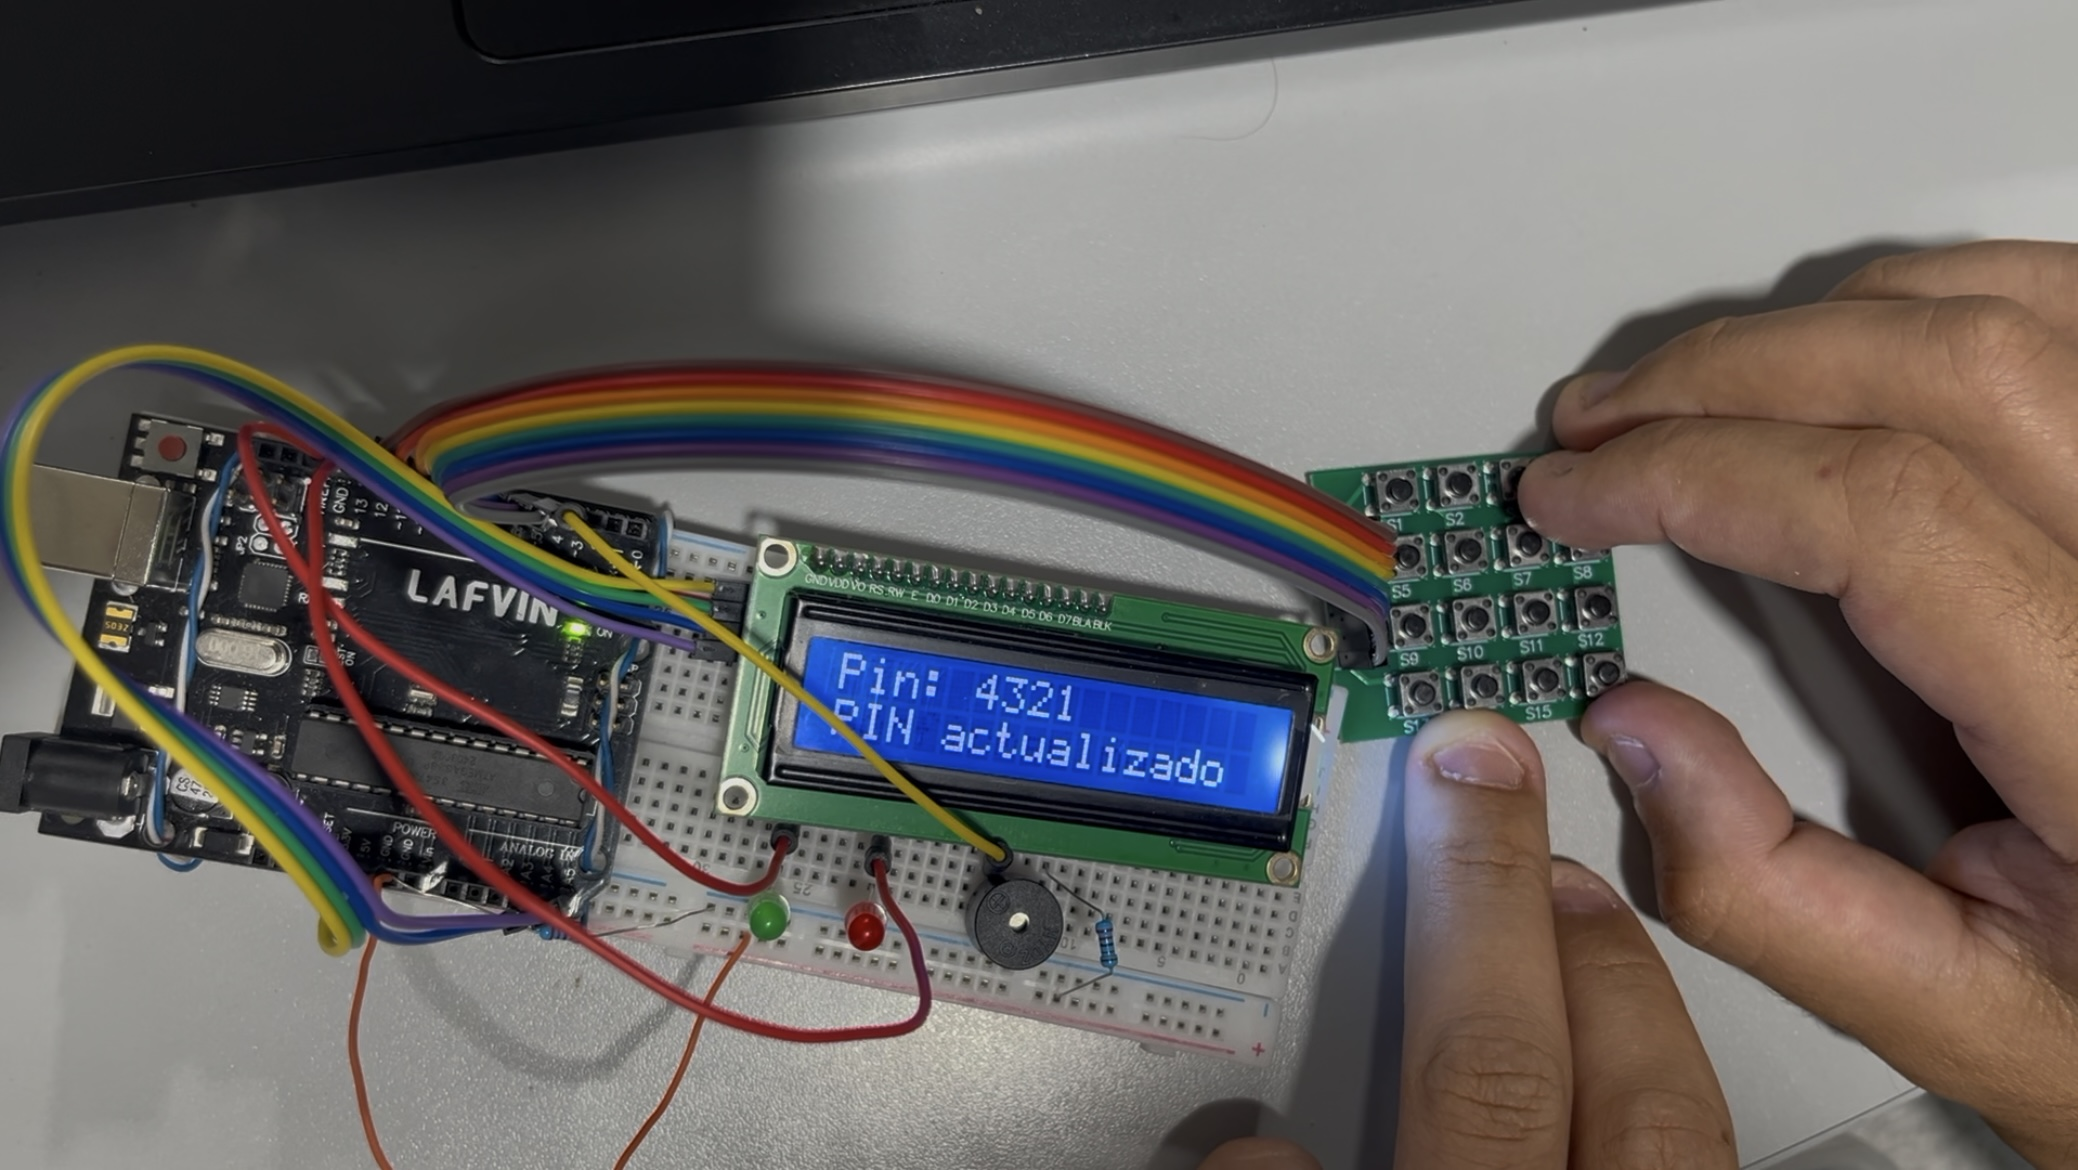
\includegraphics[width=0.7\columnwidth]{Anexos/Cerradura_PINactualizado.png}
    \caption{Proceso de cambio de PIN completado exitosamente: mensaje \texttt{PIN actualizado} en LCD y confirmación mediante LED verde y pitidos breves. Fuente: elaboración propia.}
    \label{fig:cerradura_pin_actualizado}
\end{figure}

Ante coincidencia, el nuevo valor es grabado en la EEPROM, mostrando el mensaje \texttt{PIN actualizado}, 
junto con la confirmación sonora (tres pulsos breves) y el encendido momentáneo del LED verde.  
Si los PINs no coinciden o la longitud no es válida, se muestra el error correspondiente y se enciende brevemente el LED rojo.

\subsubsection{Reinicio con tecla maestra}

Durante las pruebas del modo de bloqueo, se comprobó el correcto funcionamiento de la tecla maestra \texttt{D}, 
la cual permite reiniciar el sistema en cualquier estado.  
Al ser presionada, se apagan las señales de error o alarma, se reinician los contadores de intentos, 
y se emite la secuencia de confirmación (tres pulsos cortos de buzzer y LED verde), 
mostrándose el mensaje \texttt{MASTER OK} en la pantalla.

\subsubsection{Síntesis de resultados}

El sistema respondió correctamente ante todos los escenarios previstos: 
detección de errores, bloqueo, cambio de clave, reinicio y validación.  
La coordinación entre las salidas luminosas, sonoras y visuales permitió una retroalimentación clara al usuario, 
y la persistencia del PIN en EEPROM aseguró la conservación de la configuración entre reinicios.  
No se detectaron fallos de lectura ni errores en la escritura de memoria, 
confirmando la robustez del diseño implementado.
